\section{Gaussian Process Regression} \label{sec:gpr}
The basic building block of the multi-fidelity framework is Gaussian Process (GP) regression \cite{rasmussen_gaussian_2006}. It is a supervised learning technique used to build a surrogate model for an unknown function $y = f(\mathbf{x})$ given $n$ observed input-output pairs $\mathcal{D} = \{\mathbf{x}_i, y_i\}$ for $i \in\{1,...,n\}$. The function can be non-deterministic and have noise, $\sigma$, associated with its observations. In the context of this work, the computer simulations are deterministic but have modeling errors that are treated as noise in the function of interest. The unknown function can have multi-dimensional inputs, but must have a scalar output. These input-output pairs can be arranged in matrices $X$ and $\mathbf{y}$. If the function has an $m$ dimensional input then $X$ is an $\left (n \times m \right)$ matrix of inputs and $\mathbf{y}$ is an $\left (n \times 1 \right)$ vector of outputs.

Since these observations can be imperfect, each observation is assumed to carry some Gaussian noise associated with it such that $y_i \sim \mathcal{N}(E(f(\mathbf{x_i})),\sigma_i^2)$. Assuming that all the observations in $\mathcal{D}$ have a joint Gaussian distribution, a GP can be used as a surrogate model for the data. A GP is completely defined by its mean function, $ \mu(\mathbf{x}) $, and a kernel function, $\mathbf{k}(\mathbf{x,x';\theta})$, that is parameterized by some hyperparameters $\theta$. For the purposes of this study, the squared exponential function is used as the kernel function: 
\begin{equation}
    \mathbf{k}\left (\mathbf{x,x'} \right ) = \sigma_f^2 \exp \left ( -\sum_{d=1}^{d=m}\frac{\left ( x_d - x'_d \right )^2}{2l_d} \right ),
\end{equation}
where $m$ is the dimension of the input. The hyperparameters for this kernel function are the signal variance $\sigma_f^2$ and the length scales $l_d$. The kernel function is used to create a kernel matrix $K \in \mathbb{R} ^{ n \times n}$ where $K_{ij} = \mathbf{k \left( x_i, x_j \right )}$.

To enable the GP to estimate functions with a non-zero mean, the mean of $f(\mathbf{x})$ is represented using $p$ fixed basis functions, $\mathbf{h(x)}$, and learned regression coefficients $\beta$. At a minimum, these basis functions include a constant term, but can have multiple polynomial terms. With these in mind, the surrogate model $Z$ evaluated at some location of interest, $\mathbf{x}_*$, can be represented as some mean value plus a zero-mean GP: 
\begin{equation}
    Z(\mathbf{x}_*) = \mathbf{h(\mathbf{x}_*)}^T\beta + \mathcal{GP}(0,K(\mathbf{x}_*,\mathbf{x}_*';\theta)).
\end{equation}
The $n_*$ sample locations and the basis functions can also be arranged in matrices $X_* \in \mathbb{R} ^{ n_* \times m}$ and $H \in \mathbb{R} ^{ p \times n_*}$ such that each row of $X_*$ is a $m$-dimensional sample location and each column of $H_*$ is a $p$-dimensional result of the basis functions at the locations in $X_*$.

Combining the GP regression equations for noisy observations with those incorporating explicit basis functions, and writing in the matrix notation, the surrogate model is defined as 
\begin{equation}
    Z(X_*) \sim \mathcal{GP} (\mu(X_*), \sigma^2(X_*,X_*)),
\end{equation}
\begin{equation} \label{equ:mu_gpr}
    \mu(X_*) = H_*^T\hat{\beta} + K(X_*,X)[K(X,X)+\text{diag}(\sigma_i)]^{-1} (y-H^T\hat{\beta}), 
\end{equation}
\begin{equation} \label{equ:sig_gpr}
    \sigma^2(X_*,X_*) = K(X_*,X_*) - K(X_*,X)[K(X,X)+\text{diag}(\sigma_i)]^{-1} K(X,X_*), 
\end{equation}
where $\hat{\beta} = (H^TV^{-1}H)^{-1}H^TV^{-1}y$ is the best linear estimator for the basis coefficients and $V = K(X,X) + \text{diag}(\sigma_i)$ represents the kernel matrix at the observed points $\left ( K(X,X) \right )$ and includes the Gaussian noise that is associated with each observation $\left ( \sigma_i \right )$. The prediction from the surrogate model $Z(X_*)$ is defined by the mean $\mu(X_*)$ and the uncertainty associated with these predictions is represented by the diagonal of the $\sigma^2(X_*,X_*)$ function. To fully define the GP, the hyperparameters of the kernel function need to be learned from the data. The hyperparameters are chosen by maximizing the marginal log-likelihood of the model, 

\begin{equation}
    \log~p(y|x;\theta) = -\frac{1}{2} \log|V| - \frac{1}{2}\alpha^T V^{-1}\alpha - \frac{n}{2}\log 2\pi,
\end{equation}
where $\alpha = \left ( y-H^T\hat{\beta} \right )$.

For consistency across sections, the following low- and high-fidelity analytic functions will be used to show the functioning of the GP regression process: 
\begin{align} \label{equ:lf_function}
    f_{LF}(x) &= 0.5 \left ( 6x - 2\right )^2 \sin{ \left (12x -4 \right )} + 10 \left ( x - 0.5 \right ) -5.
\\ \label{equ:hf_function}
    f_{HF}(x) &= 2 f_{LF}(x) - 20x + 20 + \sin {\left ( 10 \cos{ \left ( 5x \right )}\right )}.
\end{align}

To show a basic example of how single-fidelity GP regression uses discrete function evaluations to create a continuous representation of the QoI, only the high fidelity function is used.
Figure \ref{fig:gpr_predictions} shows the GP regression results when using 8 discrete data points to estimate the function defined by Equation \ref{equ:hf_function}.
The data points are uniformly distributed between $0$ and $1$.
In the case of Figure \ref{subfig:gpr_deterministic}, the function evaluations are considered exact, with no associated uncertainty ($\sigma_i = 0$). 
The error estimate from the GP regression goes to zero near these data points, but increases between them where there is greater uncertainty in the underlying function. 
Figure \ref{subfig:gpr_uncertain} assumes that there is uncertainty associated with the function evaluations ($\sigma_i = 1.0$).
The GP regression respects this uncertainty in the data and the error estimate incorporates it into the prediction of the underlying function, even at the data locations. 

\begin{figure}
    \centering
    \begin{subfigure}[\label{subfig:gpr_deterministic} With deterministic inputs.] {
        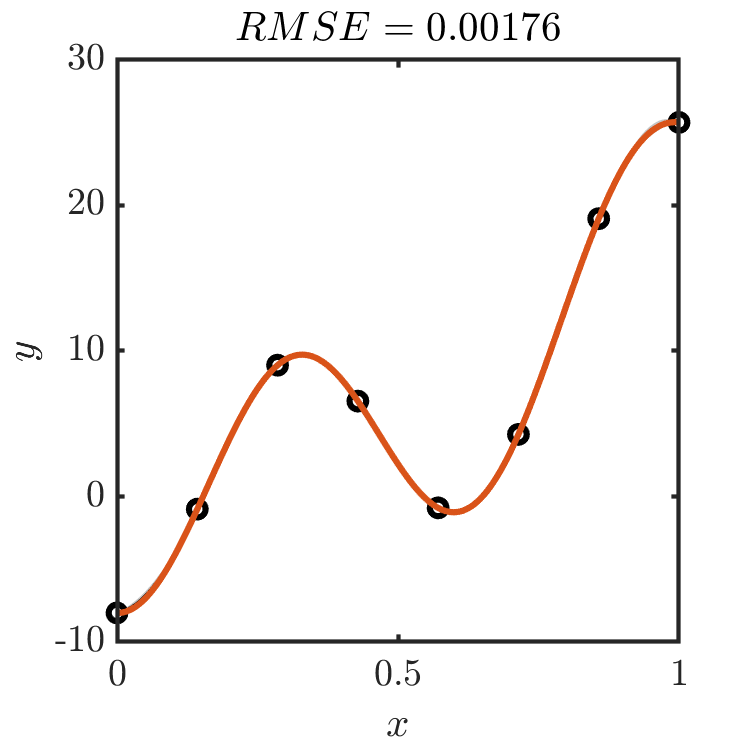
\includegraphics[width=.45\textwidth]{code/image_gen/gp_analytical/images/hf_8.png} }
    \end{subfigure}
    \hfill
    \begin{subfigure}[\label{subfig:gpr_uncertain} With uncertain inputs.]{
        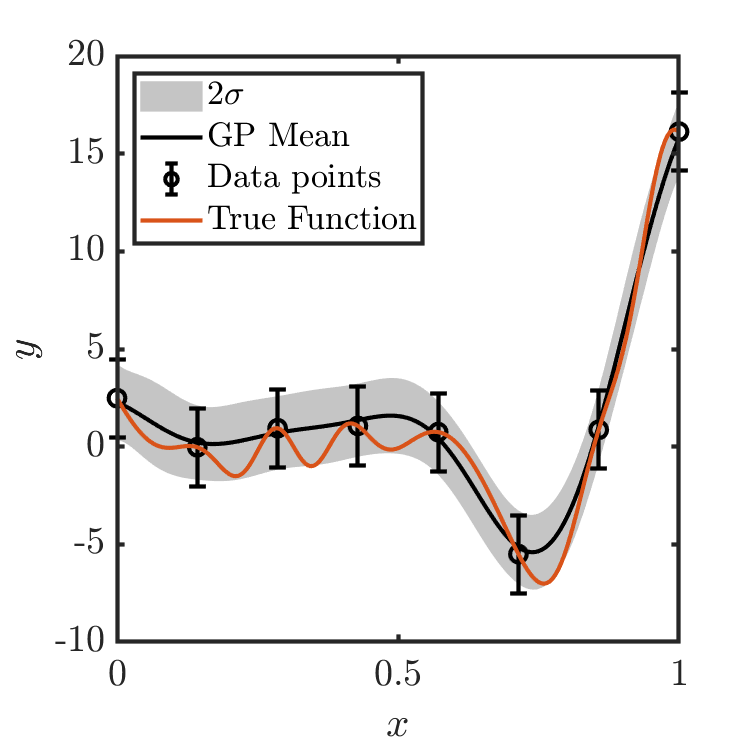
\includegraphics[width=.45\textwidth]{code/image_gen/gp_analytical/images/hf_8_noise.png} 
    }
    \end{subfigure}
    \caption{ GP regression mean and $2\sigma$ error estimates when using deterministic and uncertain input data for an underlying analytic function of interest. \label{fig:gpr_predictions}}
\end{figure}

